% !TEX root = Slide.tex

\title{Pelican e perchè generare\\ siti statici}
\subtitle{senza farsi del male}
\author{Matteo Scarpa \\ @fundor333}
\institute{Pycon 9}


\begin{document}
\frame{\maketitle}

\begin{frame}
	\frametitle{Chi sono}
	\begin{columns}
		\column{0.5\textwidth}
		\begin{itemize}
			\item Informatico e Pythonista
			\item Sostenitore dell'Open Source
			\item Stalker di Python Italia, Gdg Venezia, DataBeers Venezia
			\item @Fundor333
		\end{itemize}
		\column{0.5\textwidth}
		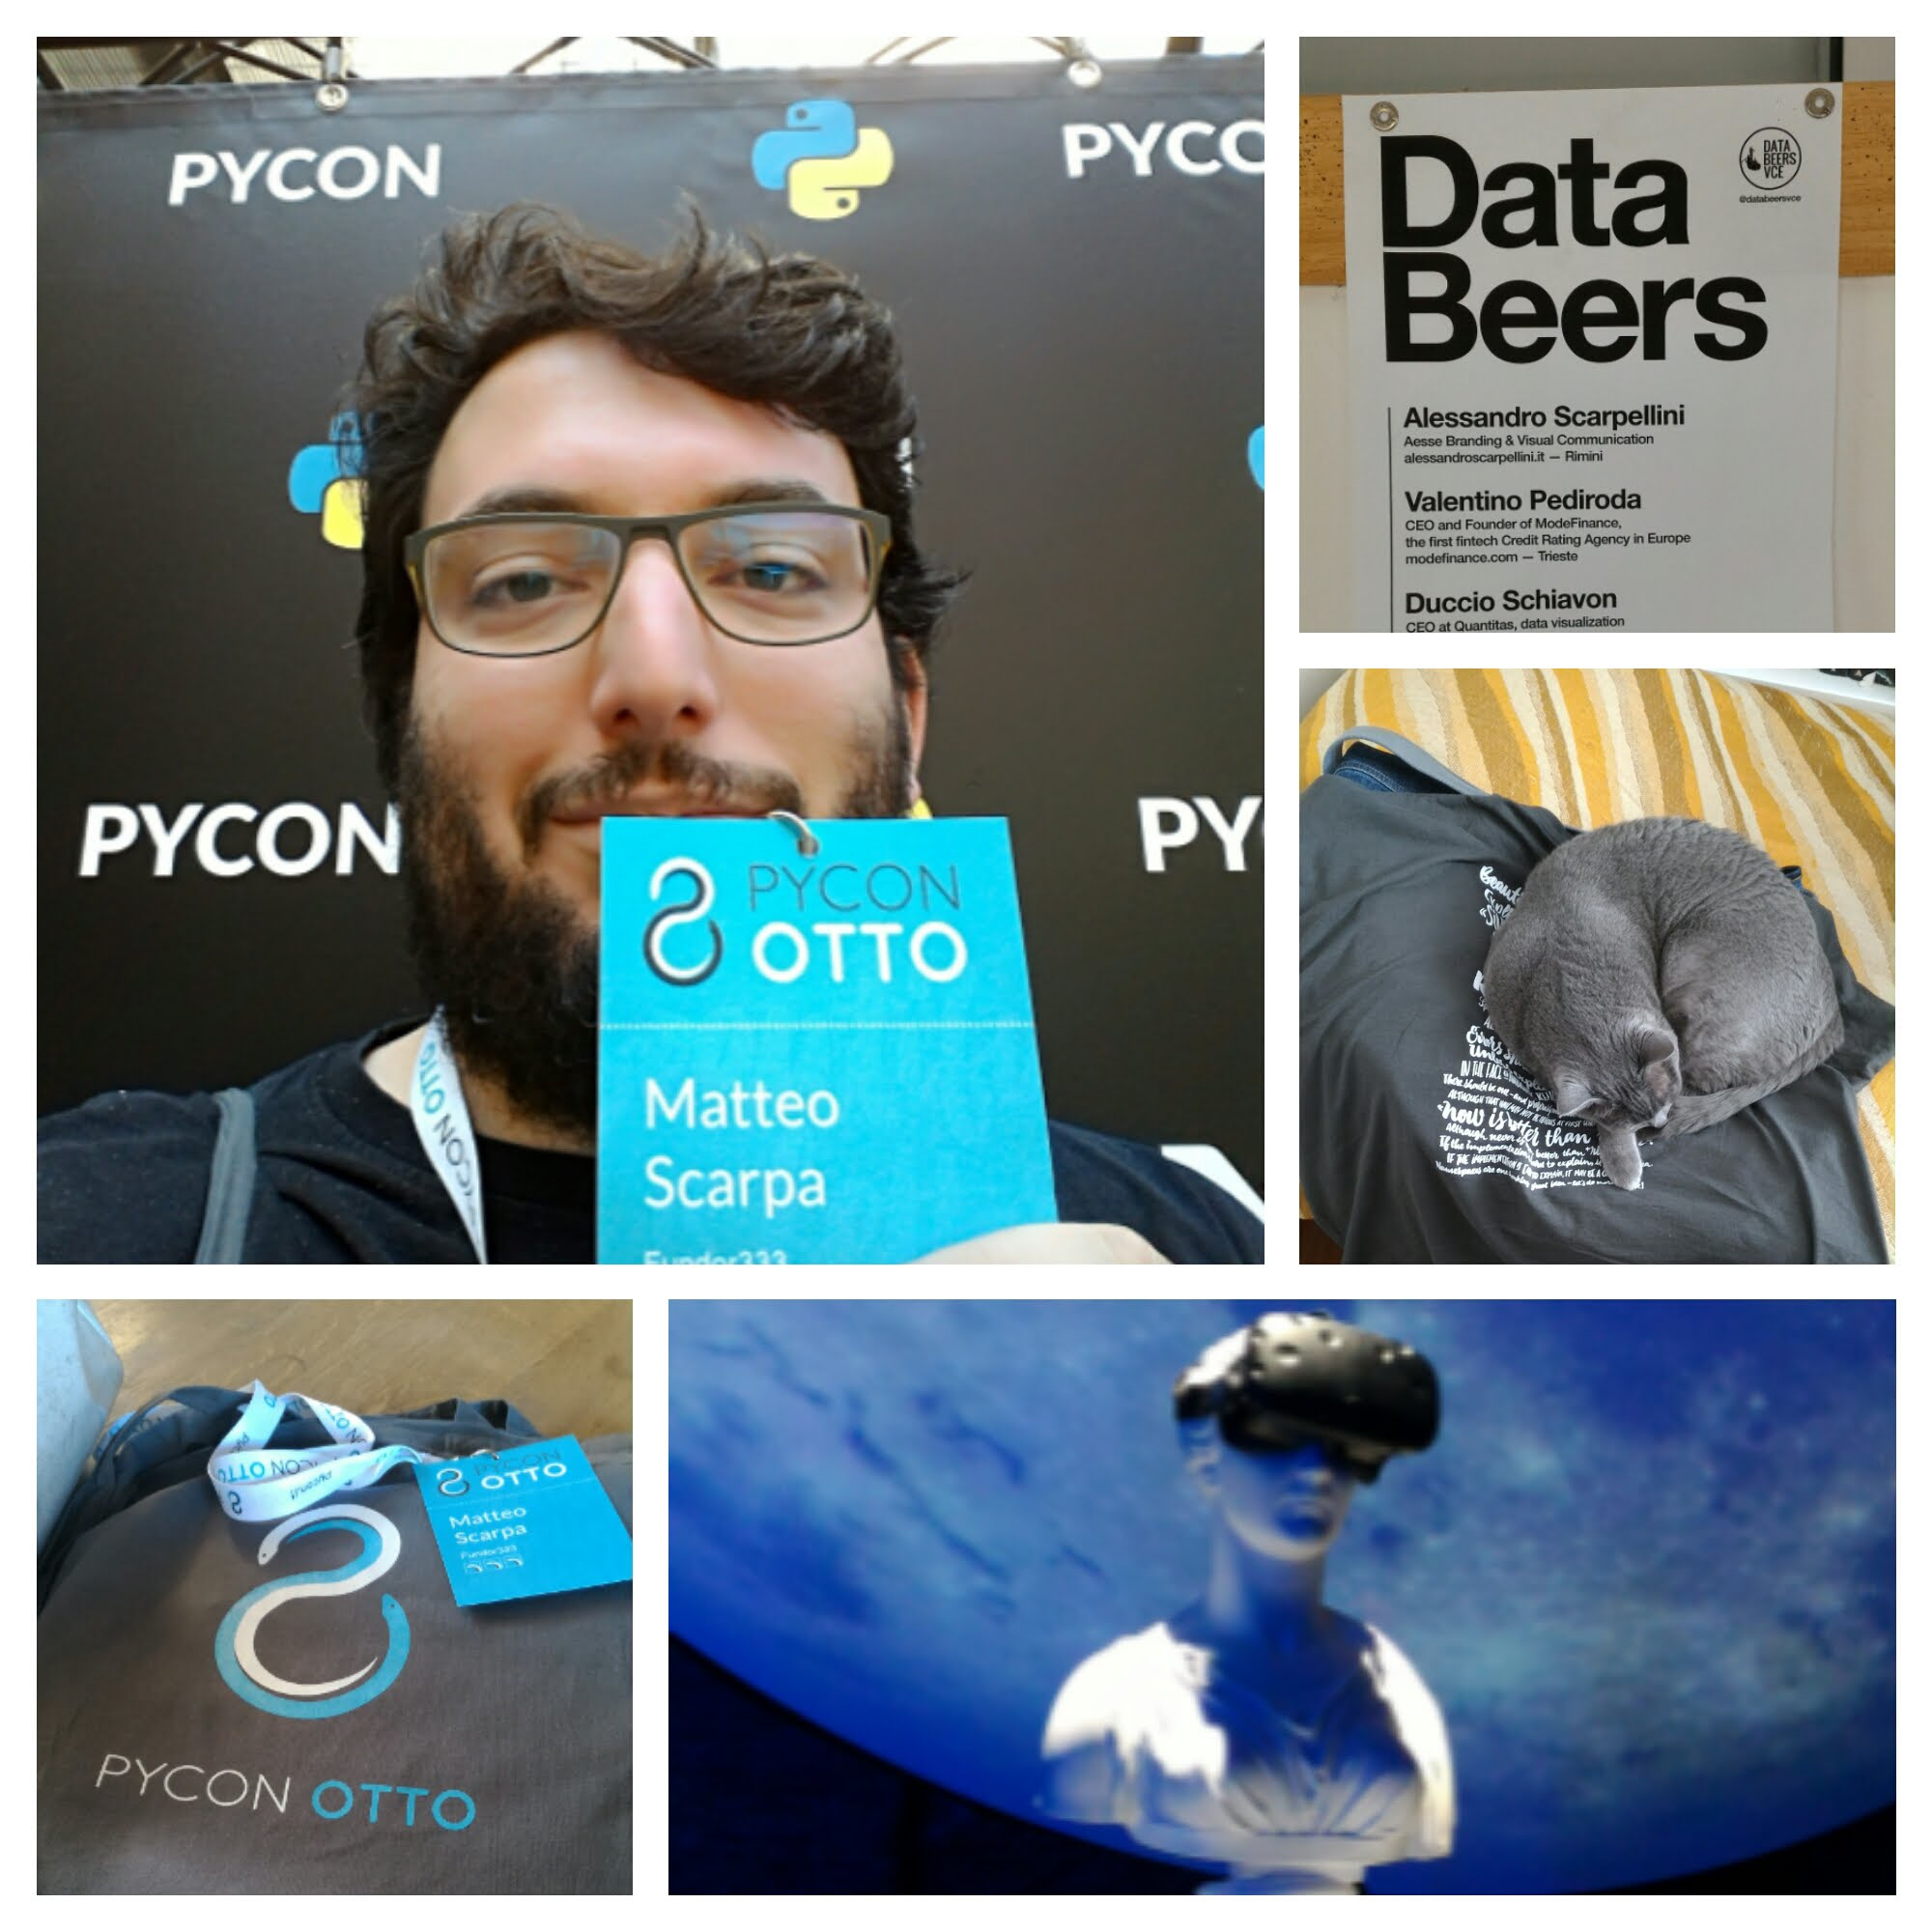
\includegraphics[scale=0.08]{img/foto}
	\end{columns}
\end{frame}

\begin{frame}
	\frametitle{Attenzione}
	\begin{center}
		
\includegraphics[scale=0.5]{img/pillole}
	\end{center}

\end{frame}


\begin{frame}
	\frametitle{Dizionario}
	\begin{itemize}
		\item \textbf{Python}: Python 3.x
		\item \textbf{Legacy Python}: Python 2.7.x
		\item \textbf{CSM}: Content Management System
		\item \textbf{Sito}: Quello che voglio ottenere
		\item \textbf{Utente}: Utilizzatore del sito e fonte dei problemi
	\end{itemize}
\end{frame}

\begin{frame}
	\frametitle{<Inserisci nome del CMS>}
	\framesubtitle{Componenti di base}
	\begin{itemize}
		\item<2-> Software lato server
		\item<3-> Database con i contenuti
		\item<4-> Backend accessibile via account/password
		\item<5-> Plugin per funzionalità
	\end{itemize}
\end{frame}

\begin{frame}
	\frametitle{Vantaggi e svantaggi di un CMS}
	\begin{columns}
		\column{0.5\textwidth}

		\textbf{Vantaggi}
		\begin{itemize}
			\item<2-> Possibile aggiornare sito da internet
			\item<3-> Solitamente semplice da usare
			\item<4-> Estendibile attraverso plugins
		\end{itemize}

		\column{0.5\textwidth}

		\textbf{Svantaggi}
		\begin{itemize}
			\item<2-> Soggetto a password fragili
			\item<3-> Più è conosciuto più è sotto attacco
			\item<4-> Da mantenere aggiornato per evitare bug o buchi
		\end{itemize}

	\end{columns}
\end{frame}

\begin{frame}
	\frametitle{Static Site Generator}
	\begin{itemize}
		\item<1-> Software che genera HTML
		\item<2-> Contenuto in file statici
		\item<3-> Va lanciato con modifiche al contenuto
	\end{itemize}
\end{frame}

\begin{frame}
	\frametitle{Pelican}
	\begin{columns}
		\column{0.5\textwidth}
		\begin{center}
		
\includegraphics[scale=0.2]{img/pelican_logo}
		\end{center}
		\column{0.5\textwidth}
		\begin{center}
		\qrcode[height=1in]{http://docs.getpelican.com/en/stable/}
		\end{center}
	\end{columns}
\end{frame}

\begin{frame}
	\frametitle{Le funzionalità di Pelican}

	\begin{columns}
			\column{0.5\textwidth}
	\begin{center}
	
\includegraphics[scale=0.2]{img/pelican_stuff}
	\end{center}
		\column{0.5\textwidth}
	\begin{itemize}
	\item Usa \textit{reStructuredText} e \textit{Jinja2}
  \item Se presente usa anche \textit{MarkDown}
  \item Elabora \textit{Jupyter Notebook} con plugin
  \item Api per aggiungere formati di file
	\end{itemize}
	\end{columns}
\end{frame}

\begin{frame}
  \frametitle{Come iniziare con Pelican}
		\begin{center}
			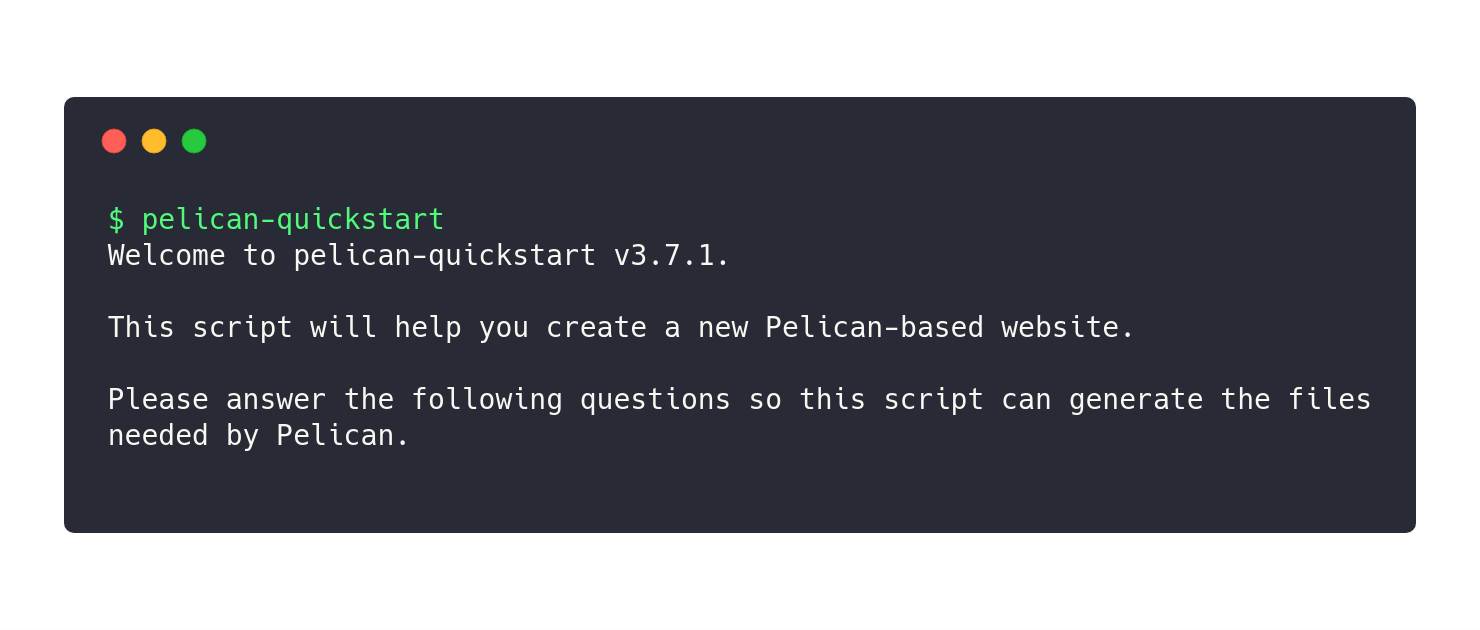
\includegraphics[scale=0.2]{img/quickstart.png}
		\end{center}  
\end{frame}


\begin{frame}
	\frametitle{Domande?}
	\begin{center}
		
\includegraphics[scale=0.15]{img/cat-with-glasses}
	\end{center}
\end{frame}

\end{document}
